\documentclass[./../../paper.tex]{subfiles}
\graphicspath{{\subfix{./../../figures/}}}

\begin{document}
\subsection{A definition for Business Processes}
Before elaborating on Process Mining, we have to establish the meaning of the term \emph{process}. The term is widely-used and therefore, has a rich semantic volume. A process generally refers to something that advances and changes over time\autocite{_DefinitionPROCESS_}.
Despite, legal or biological processes being valid interpretations, too, we focus on \emph{business processes}.

An example is a loan application process in which an applicant may request a loan. The case would then be assessed and reviewed by multiple examiners and end in a final decision. The loan might end up in an approval or denial. The \emph{business} part is misleading as these processes are not confined to commercial settings alone. For instance, a medical business process may cover a patients admission to a hospital, followed by a series of diagnostics and treatments and ending with the recovery or death of a patient. Another example from a \gls{HCI} perspective would be an order process for an online retail service like Amazon. The buyer might start the process by adding articles to the shopping cart and proceeding with specifying their bank account details. This order process would end with the submission or receival of the order.

All of these examples have a number of common characteristics. They have a clear starting point which is followed by numerous intermediary steps and end in one of the possible sets of outcomes. For this work, we mainly follow the understanding outlined in \citeauthor{vanderaalst_ProcessMiningManifesto_2012}\autocite{vanderaalst_ProcessMiningManifesto_2012}. Each step, including start- and end-points, is a \gls{event} which was caused by an \emph{activity}. Often, both terms, \emph{event} and \emph{activity}, are used interchangeably. However, there are subtle differences. We understand an event as something that happens at a specific point in time. The driving question is \emph{when} the event happens. In contrast, an activity is related to the content of an event. Here, we ask \emph{what} happens at a point in time. For instance, if we apply for a loan that requires an approval by one person and afterwards a second approval, we can call both activities \textbf{APPROVAL}. Although both activities are fundamentally the \emph{same}, they happen at different points in time. Henceforth, both events remain \emph{different}. Mainly, because one can argue that both events have varying time dependent contexts. For instance, an approval at daytime might be caused by different reasons, than an event caused at night-time.     

Each \gls{event} may contain additional information in the form of event attributes. If a collection of events \emph{sequentially} relate to a single run through a process, we call them \emph{\gls{instance}} or \emph{trace}. These instances do not have to be completed. Meaning, the trace might end prematurely. In line with the aforementioned examples, these \glspl{instance} could be understood as a single loan application, a medical case or a buy order. We can also attach \gls{instance} related information to each instance. Examples would be the applicants location, a patients age or the buyers budget. In its entirety, a business process can be summarised as a \emph{graph}, a \emph{flowchart} or another kind of visual representation. \autoref{fig:example_process}'s graphical representation is an example of such a \emph{process map}\autocite{vanderaalst_ProcessMiningManifesto_2012}. 


\begin{figure}[htb]
    \centering
    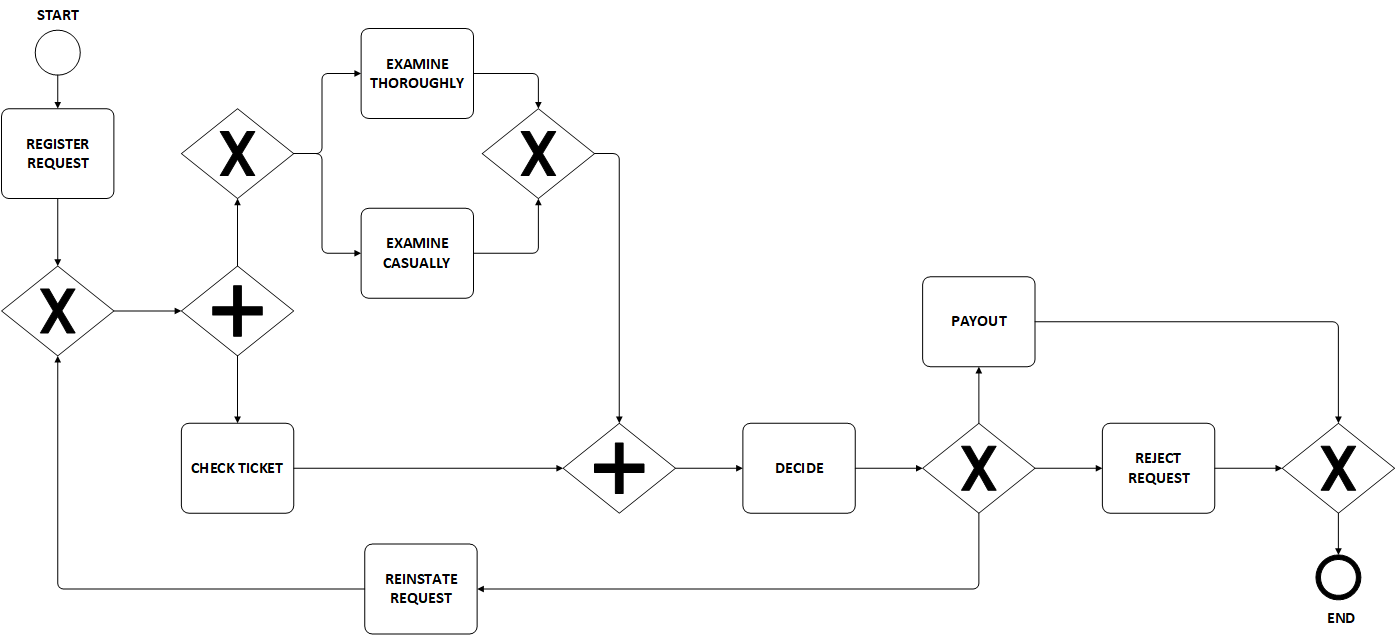
\includegraphics[width=0.99\textwidth]{figures/example_process.png}
    \caption{This graph shows an example of a \gls{BPMN} process map.}
    \label{fig:example_process}
\end{figure}



In conclusion, in this thesis a \emph{business process} refers to \begin{quote}
    \emph{A finite series of discrete events with one or more starting points, intermediary steps and end points. Each intermediate step has at least one precedent and at least one antecedent step.}
\end{quote}
However, we have to address a number of issues with this definition.

First, it excludes infinite processes like solar system movements or continuous processes such as weather changes. There may be valid arguments to include processes with these characteristics, but they are not relevant for this thesis.

Second, in each example, we deliberately used words that accentuate modality such as \emph{may}, \emph{can} or \emph{would}. It is important to understand that each process anchors its definition within an application context. Hence, what defines a business process is indisputably subjective. For instance, while an online marketplace like Amazon might be interested in the process starting from the customers first visit until the successful shipment, an Amazon vendor might only be interested in the delivery process of a product.

% TODO instead of emphasisizing true process use gloassary \gls{trueprocess}
Third, the example provided in \autoref{fig:example_process} may not relate to the \emph{real} underlying data generating process. As process \emph{models} are inherently simplified, they may or may not be accurate. The \gls{trueprocess} is often unknown. Therefore, we distinguish between the \emph{true process} and a \emph{modelled process}. The \emph{true process} is a hypothetical concept whose \emph{true} structure remains unknown. In, contrast, a process \emph{model} simplifies and approximates the characteristics of the \emph{true process}.

\subsection{What is Process Mining?}
Having established a definition for a process, we next discuss \emph{Process Mining}. This young discipline has many connections to other fields that focus on the modelling and analysis of processes such as \gls{CPI} or \gls{BPM}\autocite{vanderaalst_ProcessMiningManifesto_2012}. However, its data-centric approaches originate in \gls{DM}.
The authors \citeauthor{vanderaalst_ProcessMiningManifesto_2012} describe this field as a discipline \enquote{to discover, monitor and improve real processes (i.e., not assumed processes) by extracting knowledge from event logs readily available in today's (information) systems}\autocite{vanderaalst_ProcessMiningManifesto_2012}. The discipline revolves around the analysis of \glspl{log}.
% TODO: Minor mistake with information systems
An \gls{log} is a collection of \glspl{instance}, which are retrieved from various sources like an \gls{IS} or database. Logs are often stored in data formats such as \gls{CSV} or \gls{XES}\autocite{vanderaalst_ProcessMiningManifesto_2012}.

\subsection{The Challenges of Process Mining}
As mentioned in \autoref{sec:intro}, process data modelling and analysis is a challenging task. \citeauthor{vanderaalst_ProcessMiningManifesto_2012} mentions a number of issues that arise from processes\autocite{vanderaalst_ProcessMiningManifesto_2012}.

The first issue arises from the quality of the dataset. Process logs are seldomly collected with the primary goal of mining information and hence, often appear to be of subpar quality for information mining purposes. The information is often incomplete, due to a lack of context information, the ommision of logged process steps, or wrong levels of granularity\autocite{vanderaalst_ProcessMiningManifesto_2012}.

This issue is exacerbated by the second major issue with process data. Mainly, its complexity. Not only does a process logs' complexity arise from the variety of data sources and differing levels of complexity, but also from the datas' characteristics. The data can often be viewed as multivariate sequence with discrete and continuous features and variable length. 
This characteristic alone creates problems explored in \autoref{sec:sequences}. However, the data is also just a \emph{sample} of the process.
Hence, it may not reflect the real process in its entirety. In fact, mining techniques need to incorporate the \emph{open world assumption} as the original process may generate unseen \glspl{instance}\autocite{vanderaalst_ProcessMiningManifesto_2012}.

A third issue which contributes to the datasets' incompleteness and complexity is a phenomenon called \emph{concept drift}\autocite{vanderaalst_ProcessMiningManifesto_2012}. This phenomenon relates to the possibility of changes in the \gls{trueprocess}. The change may occur suddenly or gradually and can appear in isolation or periodically. An expression of such a drift may be a sudden inclusion of a new process step or domain changes of certain features. These changes are not uncommon and their likelihood increases with the temporal coverage and level of granularity of the dataset\autocite{vanderaalst_ProcessMiningManifesto_2012}. In other words, the more \emph{time} the dataset covers and the higher its detail, the more likely a change might have occurred over the time.

All three issues relate to the \emph{representativeness} of the data with regards to the unknown \gls{trueprocess} that generated the data. However, they also represent open challenges that require research on their own. For our purpose, we have to assume that the data is representative and its underlying process is static. These assumptions are widely applied in the body of process mining literature\autocites{tax_PredictiveBusinessProcess_2017a,klimek_Longtermseriesforecasting_2021}.
\end{document}